\section{Le laser}
Le mot \textbf{laser} est une abréviation anglo-saxonne signifiant
\textit{Light Amplification by Stimulated Emission of Radiation}. Quel que soit
le type de laser, un laser est constitué de trois éléments : un amplificateur de
lumière utilisant l'émission stimulée, un résonateur optique, et un couplage
avec l'extérieur. Les premiers oscillateurs --- et résonateurs --- sont
essentiellement les cavités (ou interféromètres) de Fabry--Perot et furent
construits en 1890 à l'aide de deux miroirs plans se faisant face. La mise au
point de l'amplificateur s'échelonna de 1917 (postulat de l'émission stimulée
par Einstein) à 1950 (pompage optique de Kastler). La première réalisation d'un
laser date de 1960 (Maiman).

Un système amplificateur est, dans le cas général, un système qui lorsqu'il est
soumis à un champ oscillant de fréquence $\nu$ et d'amplitude $E_{in}$ fournit
à sa sortie un champ dont l'amplitude et la phase ont été modifiées :
\[E_{out}=\sqrt{G}\,e^{i\varphi}E_{in},\]
avec $G$ le gain de l'amplificateur et $\varphi$ son déphasage. What makes the
optical case special is the mechanism behind the gain. Cette amplification est
basée sur le phénomène d'\textbf{émission stimulée} (\textit{stimulated
emission}) ou émission induite, caractéristique essentielle de l'interaction
entre un système matériel quantique (atomique, moléculaire, semi-conducteur…) et
le rayonnement électromagnétique. Pour bien comprendre l'émission stimulée, il
est essentiel de revenir au principe général d'émission de lumière. Puis, nous
nous attarderons sur un type d'émission, la luminescence. Nous verrons ensuite
le fonctionnement des amplificateurs de lumière utilisant le principe de
l'émission stimulée pour enfin décrire le fonctionnement d'un laser.

\subsection{Principe de l'émission de lumière}
Si l'on revient sur les constituants de la matière, on sait qu'elle est faite
d'assemblage d'atomes parfois assemblés sous forme de molécules et que ces
atomes sont eux-mêmes constitués de particules subatomiques qui pour certaines
sont chargées positivement (protons) et d'autres négativement (électrons). La
lumière est un phénomène physique de transport d'énergie sans transport de
matière qui consiste en la génération d'un champ électromagnétique oscillant
temporellement tout en se propageant spatialement.

Pour générer une onde électromagnétique qui se propage, il suffit donc de faire
osciller une particule chargée (que l'on considérera comme un dipôle) à la
fréquence désirée. L'émission de lumière se fait donc sous l'action d'une
perturbation électromagnétique qui fait vibrer l'atome, initialement dans un
état excité $\ket{b}$, et le couple avec un autre état de moindre énergie
$\ket{a}$. Pendant le changement d'état de $\ket{b}$ vers $\ket{a}$, l'atome se
comporte comme une antenne et rayonne un champ. Celui-ci transporte l'énergie
perdue par l'atome.

\begin{example}[Radio-frequency antennas]
  C'est comme ceci que l'on génère par exemple une onde radio-fréquence en
  appliquant à un conducteur un courant alternatif. De la même manière, pour une
  antenne réceptrice, c'est cette fois le champ électromagnétique incident qui
  fait osciller un dipôle de l'antenne qui, à son tour, va générer un courant
  alternatif portant l'information sur le signal.
\end{example}

Il convient de classer l'émission de lumière en trois domaines dont les
caractéristiques spectrales, temporelles et spatiales sont bien différentes :
le \textbf{rayonnement thermique} (\textit{thermal radiation}), la
\textbf{luminescence}, et le \textbf{rayonnement stimulé} (\textit{stimulated
radiation}), which is the laser.

\subsection{Le rayonnement thermique}
La température d'un corps est liée à l'agitation des molécules et des atomes et
des particules qui les forment. Or, les charges électriques en mouvement
émettent des ondes électromagnétiques. Donc, \emph{tout} corps porté à une
certaine température émet des ondes EM, c'est ce que l'on appelle le
rayonnement thermique. C'est Planck qui a mis en équation ces émissions
lumineuses d'origine thermique. Sans rentrer dans les détails, which are beyond
this course, il a montré que les caractéristiques de ce rayonnement dépendent
de la température. Notamment,
la loi de Planck déduite de la loi de Wien (courtes longueurs d'onde) et la loi
de Rayleigh--Jeans (grandes longueurs d'onde) montrent que la longueur d'onde
centrale du spectre d'émission est inversement proportionnelle à la
température. Ainsi, un corps qui rayonne dans le rouge est \emph{plus froid}
qu'un corps qui rayonne dans le bleu (même si le code couleur des robinetteries
indique le contraire).

\begin{theorem}[Loi de Planck (\textit{Planck's law}), 1901]
  Dans le cas d'un grand nombre de particules indiscernables, la densité
  volumique et spectrale d'énergie $\rho_\nu$ (énergie par unité de volume et
  unité de fréquence) du rayonnement thermique est
  \[\rho_\nu=\frac{8\pi h\nu^3}{c^3}\,\frac{1}{e^{h\nu/k_BT}-1},\]
  avec $k_B$ la constante de Boltzmann.
\end{theorem}

\begin{figure}[h!]
  \centering
  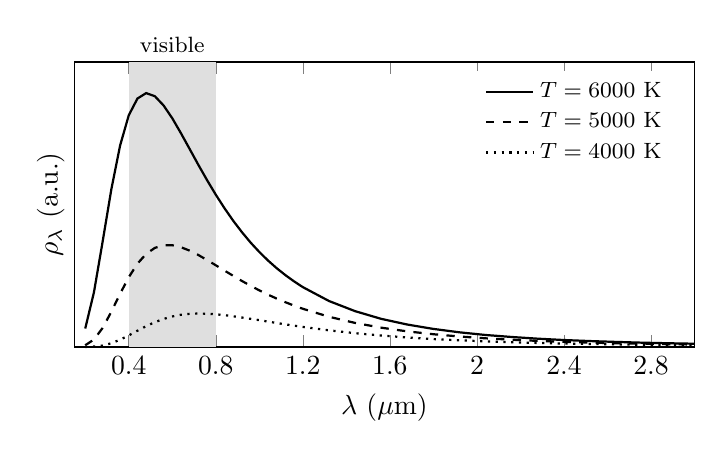
\begin{tikzpicture}
    \begin{axis}[width=0.78\textwidth, height=5.2cm,
      xlabel={$\lambda$ ($\mu$m)}, ylabel={$\rho_\lambda$ (a.u.)},
      xmin=0.15, xmax=3, ymin=0, ymax=0.30,
      ytick=\empty, xtick={0.4,0.8,1.2,1.6,2,2.4,2.8},
      legend pos=north east, legend cell align=left,
      legend style={draw=none, font=\footnotesize}, clip=false,
      every axis plot/.append style={thick}]
      \fill[gray!25] (axis cs:0.4,0) rectangle (axis cs:0.8,0.30);
      \node[font=\footnotesize, anchor=south] at (axis cs:0.6,0.30) {visible};
      \addplot[black] coordinates {(0.200,0.0194) (0.240,0.0575) (0.280,0.1109)
        (0.320,0.1660) (0.360,0.2119) (0.400,0.2439) (0.440,0.2616)
        (0.480,0.2673) (0.520,0.2640) (0.560,0.2543) (0.600,0.2408)
        (0.640,0.2250) (0.680,0.2084) (0.720,0.1917) (0.760,0.1756)
        (0.800,0.1603) (0.840,0.1461) (0.880,0.1329) (0.920,0.1209)
        (0.960,0.1099) (1.000,0.1000) (1.040,0.0910) (1.080,0.0829)
        (1.120,0.0756) (1.160,0.0690) (1.200,0.0630) (1.320,0.0484)
        (1.440,0.0377) (1.560,0.0296) (1.680,0.0236) (1.800,0.0190)
        (1.920,0.0154) (2.040,0.0126) (2.160,0.0105) (2.280,0.0087)
        (2.400,0.0073) (2.520,0.0062) (2.640,0.0053) (2.760,0.0045)
        (2.880,0.0039) (3.000,0.0034)};
      \addlegendentry{$T=6000$ K}
      \addplot[black, dashed] coordinates {(0.200,0.0018) (0.240,0.0078)
        (0.280,0.0200) (0.320,0.0371) (0.360,0.0559) (0.400,0.0734)
        (0.440,0.0877) (0.480,0.0980) (0.520,0.1043) (0.560,0.1071)
        (0.600,0.1071) (0.640,0.1050) (0.680,0.1014) (0.720,0.0968)
        (0.760,0.0915) (0.800,0.0860) (0.840,0.0804) (0.880,0.0749)
        (0.920,0.0695) (0.960,0.0644) (1.000,0.0596) (1.040,0.0551)
        (1.080,0.0509) (1.120,0.0471) (1.160,0.0435) (1.200,0.0402)
        (1.320,0.0318) (1.440,0.0253) (1.560,0.0203) (1.680,0.0164)
        (1.800,0.0134) (1.920,0.0110) (2.040,0.0091) (2.160,0.0076)
        (2.280,0.0064) (2.400,0.0054) (2.520,0.0046) (2.640,0.0039)
        (2.760,0.0034) (2.880,0.0029) (3.000,0.0026)};
      \addlegendentry{$T=5000$ K}
      \addplot[black, dotted] coordinates {(0.200,0.0000) (0.240,0.0004)
        (0.280,0.0015) (0.320,0.0039) (0.360,0.0076) (0.400,0.0121)
        (0.440,0.0171) (0.480,0.0219) (0.520,0.0261) (0.560,0.0295)
        (0.600,0.0321) (0.640,0.0339) (0.680,0.0349) (0.720,0.0352)
        (0.760,0.0350) (0.800,0.0344) (0.840,0.0335) (0.880,0.0323)
        (0.920,0.0310) (0.960,0.0296) (1.000,0.0282) (1.040,0.0267)
        (1.080,0.0252) (1.120,0.0238) (1.160,0.0224) (1.200,0.0211)
        (1.320,0.0175) (1.440,0.0145) (1.560,0.0120) (1.680,0.0100)
        (1.800,0.0083) (1.920,0.0070) (2.040,0.0059) (2.160,0.0050)
        (2.280,0.0042) (2.400,0.0036) (2.520,0.0031) (2.640,0.0027)
        (2.760,0.0023) (2.880,0.0020) (3.000,0.0018)};
      \addlegendentry{$T=4000$ K}
    \end{axis}
  \end{tikzpicture}
  \caption*{\footnotesize Densité spectrale de puissance d'une source thermique
  en fonction de la longueur d'onde pour différentes températures. The peak
  moves towards short longueurs d'onde as $T$ rises, and the spectrum is
  continuous and several hundred THz wide.}
\end{figure}

Une des principales caractéristiques du rayonnement thermique est d'être
complètement \emph{désordonné} : émission dans toutes les directions, sur un
spectre continu de fréquences, pas de relation de phase entre les différents
photons émis. En termes plus scientifiques, on dira que le rayonnement
thermique est \textbf{incohérent}. Ce type d'émission s'effectue sur un spectre
très large de plusieurs centaines de téra-Hertz (plusieurs micromètres en
longueur d'onde dans le vide), bien loin des caractéristiques des lasers et même
des diodes électroluminescentes. Ainsi le soleil émet non seulement un spectre
dans l'ensemble du visible mais également dans l'UV et l'IR.

\begin{example}[Everyday thermal sources]
  Dans notre quotidien, les sources de lumière sont en général produites par un
  rayonnement thermique. L'exemple le plus évident est le soleil mais l'ampoule
  à incandescence, le métal chauffé, le métal en fusion et même un corps humain
  émettent ce type de lumière (la longueur d'onde d'émission d'un corps humain
  étant autour de $10\ \mu$m) --- the emission a thermal camera records.
\end{example}

\begin{remark}[Thermodynamic equilibrium]
  À l'équilibre thermodynamique, état atteint par le système si on le laisse
  évoluer suffisamment longtemps sans apport d'énergie provenant de
  l'extérieur, les niveaux d'énergie ont une occupation moyenne qui décroit avec
  la valeur de l'énergie et ce d'autant plus rapidement que la température est
  basse. Lorsqu'il part d'un état initial hors équilibre contenant donc des
  constituants excités (atomes, molécules, …), le système va évoluer en
  permettant aux constituants de perdre leur énergie excédentaire, énergie qui
  sera soit évacuée par rayonnement d'onde électromagnétique, soit conservée
  dans le système sous forme de chaleur contribuant à fixer la température
  finale du système.
\end{remark}

\subsection{Les transitions radiatives : la luminescence}
Il existe d'autres manières d'émettre de la lumière. Ainsi, la lumière émise par
luminescence résulte de transitions atomiques entre deux états d'énergie
\emph{discrets} d'un atome ou d'une molécule. Ces transitions génèrent un
échange d'énergie $E_b-E_a$ qui peut s'effectuer de deux manières : dans la
plupart des cas de manière \textbf{non radiative}, sans émission ni absorption
de lumière, libérant alors dans le matériau de l'énergie cinétique sous forme de
\textbf{phonon} (quantum d'énergie de vibration du cristal) ; dans certains cas,
la transition est \textbf{radiative} et s'accompagne de l'absorption ou de la
génération d'un photon. C'est ce cas qui naturellement nous intéresse.

Considérons un système atomique à deux niveaux d'énergie $E_a$ et $E_b$. Les
atomes présents dans le matériau se trouvent dans l'un ou l'autre de ces états.
Nous appellerons $N_a$ la \textbf{population} du niveau $E_a$ qui sera considéré
comme niveau fondamental du système (nombre d'atomes par unité de volume dans
l'état $E_a$) et $N_b$ la population du niveau $E_b$. Entre ces niveaux sont
possibles des transitions radiatives correspondant à des photons de fréquences
$\nu_{ab}=(E_b-E_a)/h$. En 1917, Einstein montre qu'il existe trois types de
transitions entre niveaux d'énergie atomiques : l'\textbf{émission spontanée}
(\textit{spontaneous emission}), que l'on retrouve dans le cas des diodes
électroluminescentes, et les \textbf{transitions induites} (\textit{induced
transitions}) parmi lesquelles on distingue l'absorption stimulée et l'émission
stimulée, utilisée dans les lasers mais également dans les amplificateurs de
lumière.

\begin{figure}[h!]
  \centering
  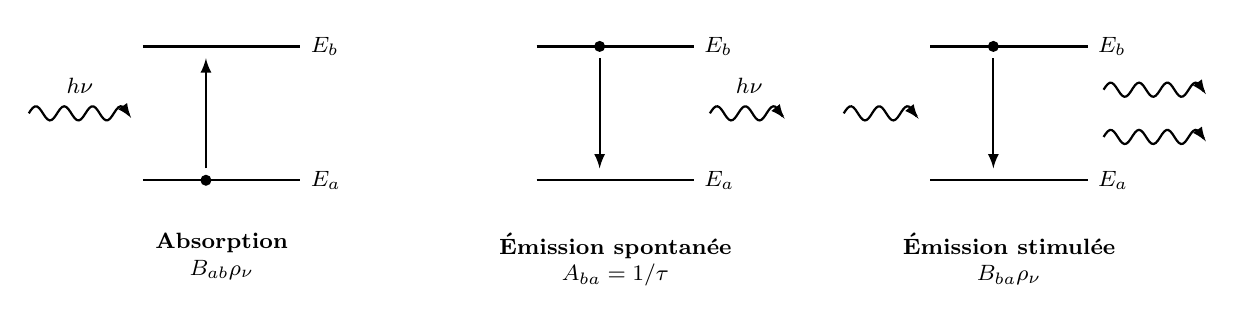
\begin{tikzpicture}[>=latex, every node/.style={font=\footnotesize}]
    \foreach \x in {0,5,10}{
      \draw[thick] (\x,0) -- (\x+2,0) node[right] {$E_a$};
      \draw[thick] (\x,1.7) -- (\x+2,1.7) node[right] {$E_b$};
    }
    % absorption
    \fill (0.8,0) circle (2pt);
    \draw[->, thick] (0.8,0.15) -- (0.8,1.55);
    \draw[->, thick] plot[domain=0:1.3, samples=50]
      ({-1.45+\x},{0.85+0.09*sin(\x*1000)});
    \node[anchor=south] at (-0.8,0.98) {$h\nu$};
    \node[anchor=north, align=center] at (1,-0.55)
      {\textbf{Absorption}\\$B_{ab}\rho_\nu$};
    % spontaneous
    \fill (5.8,1.7) circle (2pt);
    \draw[->, thick] (5.8,1.55) -- (5.8,0.15);
    \draw[->, thick] plot[domain=0:0.95, samples=40]
      ({7.2+\x},{0.85+0.09*sin(\x*1000)});
    \node[anchor=south] at (7.7,0.98) {$h\nu$};
    \node[anchor=north, align=center] at (6,-0.55)
      {\textbf{Émission spontanée}\\$A_{ba}=1/\tau$};
    % stimulated
    \fill (10.8,1.7) circle (2pt);
    \draw[->, thick] (10.8,1.55) -- (10.8,0.15);
    \draw[->, thick] plot[domain=0:0.95, samples=40]
      ({8.9+\x},{0.85+0.09*sin(\x*1000)});
    \draw[->, thick] plot[domain=0:1.3, samples=50]
      ({12.2+\x},{1.15+0.09*sin(\x*1000)});
    \draw[->, thick] plot[domain=0:1.3, samples=50]
      ({12.2+\x},{0.55+0.09*sin(\x*1000)});
    \node[anchor=north, align=center] at (11,-0.55)
      {\textbf{Émission stimulée}\\$B_{ba}\rho_\nu$};
  \end{tikzpicture}
  \caption*{\footnotesize The three Einstein transitions between two levels,
  with $h\nu=E_b-E_a$ throughout. The stimulated photon is a clone of the
  incident one.}
\end{figure}

\subsubsection{Transitions spontanées}
Seul l'état fondamental est stable dans un atome. Donc, après un certain temps,
l'atome excité finit par « retomber » spontanément à l'état fondamental en
émettant un photon d'énergie $h\nu_{ab}=E_b-E_a$, comme une bille, posée sur le
bord d'une baignoire, finirait, au moindre bruit ambiant, par retomber au fond
de cette dernière, spontanément.

\begin{definition}[Émission spontanée]
  Les émissions spontanées de photons par un ensemble d'atomes n'ont
  \emph{aucune corrélation} entre elles. Ces photons sont donc émis dans toutes
  les directions et n'ont pas de relation de phase entre eux tout comme le cas
  du rayonnement thermique : ils ne sont pas cohérents. Einstein note $A_{ba}$
  la probabilité (par atome et unité de temps) de ce phénomène.
\end{definition}

Contrairement au rayonnement thermique, l'énergie du photon spontané est
\emph{quantifiée}, le spectre est donc un spectre de raies. Cependant,
l'émission spontanée est fortement influencée par l'agitation thermique mais
aussi par des collisions entre atomes et/ou l'effet Doppler. Le spectre présente
donc en général l'aspect d'un continuum ou quasi-continuum s'étalant sur
plusieurs nanomètres. The hierarchy to remember is
\[\Delta\lambda_{\text{thermal}}\;\gg\;\Delta\lambda_{\text{spontaneous}}\;\gg\;
  \Delta\lambda_{\text{laser}},\qquad
  >\!\text{a few }\mu\text{m}\;\gg\;\text{a few nm}\;\gg\;
  \text{pm to }0.01\ \text{fm}.\]

\begin{conclusion}
  L'émission spontanée, appelée également luminescence, est un rayonnement
  \emph{incohérent} émis dans toutes les directions, avec un spectre beaucoup
  plus large que celui d'un laser mais moins que le rayonnement thermique.
\end{conclusion}

Cette luminescence peut être obtenue de plusieurs manières qui dépendent bien
souvent de la façon dont on va exciter le matériau. Cette excitation est
appelée \textbf{pompage} (\textit{pumping}).

\begin{itemize}
  \item La \textbf{photoluminescence} (excitation par absorption de photons),
    par exemple dans les tubes luminescents, les colorants fluorescents, les
    azurants optiques (un agent azurant est une molécule qui absorbe les
    rayonnements électromagnétiques ultraviolets entre 300 et 400 nm de
    longueur d'onde et réémet ensuite cette énergie par fluorescence dans le
    visible entre 400 et 500 nm). Parmi les phénomènes de photoluminescence, on
    distingue d'une part la \textit{fluorescence}, photoluminescence rapide (de
    $10^{-9}$ à $10^{-6}$ secondes pour la majorité des molécules organiques) et
    d'autre part la \textit{phosphorescence}, photoluminescence lente (de
    $10^{-3}$ à $10$ secondes). La chlorophylle absorbe le rouge et nous paraît
    donc verte.
  \item La \textbf{bioluminescence} (réaction enzymatique), utilisée par les
    lucioles.
  \item La \textbf{chimiluminescence} (excitation à la suite d'une réaction
    chimique), utilisée par exemple dans les bâtons lumineux ou le luminol.
    Durant une réaction de chimiluminescence, la molécule produite par la
    réaction se trouve dans un état excité. C'est le retour à l'état fondamental
    qui provoque le phénomène par l'émission d'une onde électromagnétique.
  \item L'\textbf{électroluminescence} (excitation électrique (champ
    électrique)), utilisée dans les diodes électroluminescentes (DEL), les
    télévisions.
\end{itemize}

\paragraph{Durée de vie d'un état excité}
Une particule excitée dans l'état $E_b$ peut spontanément passer dans l'état
$E_a$ par émission spontanée. Étudions l'évolution de la population sachant
qu'à l'instant $t=0$, on a grâce à l'excitation, une population $N_b^0$ plus
grande que la population à l'équilibre thermique (prise égale à 0). Durant
l'intervalle de temps $dt$, la population diminue de la quantité :
\[dN_b=-A_{ba}N_b\,dt=-N_b\frac{dt}{\tau}.\]
C'est la loi la plus simple que l'on puisse écrire, la perte est directement
proportionnelle à la population présente et à l'intervalle de temps étudié. La
constante $A_{ba}=1/\tau$ est le \textbf{premier coefficient d'Einstein}
(\textit{first Einstein coefficient}). En intégrant cette relation, on trouve :
\[\boxed{\,N_b=N_b^0\,e^{-t/\tau}\,}\]

\begin{definition}[Durée de vie (\textit{lifetime})]
  La constante $\tau$ est la durée de vie moyenne des états excités, c'est une
  caractéristique essentielle de chaque transition. La constante $A_{ba}$ varie
  en fonction du matériau étudié mais également suivant la transition
  considérée au sein d'un même matériau. En fait cette durée de vie rend compte
  de la capacité du matériau à faire varier ses populations par exemple en
  fonction d'une perturbation extérieure.
\end{definition}

The range of $\tau$ decides what a component is good for:
\begin{itemize}
  \item la dizaine de millisecondes pour certaines terres rares (ions Erbium
    dans une matrice de silice), permettant de faire des amplificateurs
    \emph{insensibles au débit}, c'est-à-dire avec une amplification qui ne
    varie pas entre deux bits d'information différents à des fréquences
    supérieures au GHz ;
  \item des temps inférieurs à la nanoseconde comme dans les semi-conducteurs,
    permettant de faire des composants \emph{rapides}.
\end{itemize}

\paragraph{Propriété spectrale d'une émission spontanée}
Naturellement, la puissance optique émise est proportionnelle au nombre de
désexcitations depuis l'état $\ket{b}$ vers l'état $\ket{a}$ par seconde, qui
est égal au nombre de photons émis, c'est-à-dire $h\nu A_{ba}N_b(t)$. La
décroissance de la puissance dans le temps suit donc la même loi de
décroissance en $e^{-t/\tau}$. Le champ prend donc la forme :
\[E(t)=E_0\,e^{-\frac{t}{2\tau}}\,e^{-j\omega_0 t}\qquad\text{for }t\geq 0.\]
Si on regarde la répartition des fréquences de ce champ dans le domaine
spectral, cela revient à faire une transformée de Fourier, vue largement dans
le chapitre « Diffraction ». The emission spectrum of a material whose
excited-state population decays exponentially is \textbf{lorentzien}. La densité spectrale de puissance de l'émission spontanée
s'écrit donc :
\[S_E(\omega)=\left|\mathcal{TF}[E(t)]\right|^2=E(\omega)E^*(\omega)
  =\frac{E_0^2}{\left(1/2\tau\right)^2+\left(\omega-\omega_0\right)^2}.\]
C'est une lorentzienne centrée sur la fréquence $\nu_0=\omega_0/2\pi$; its half
width at half maximum is
\[\Delta\omega=2\pi\Delta\nu=\frac{1}{2\tau}.\]

\begin{remark}
  The value $1/2\tau$ is a half width, not the \emph{total} width at half
  maximum: $S_E$ falls to half its maximum at $\omega-\omega_0=\pm 1/2\tau$, so
  $1/2\tau$ is the half width at half maximum and the full width is $1/\tau$.
  Keep this convention, but remember the factor 2 whenever a full width is
  wanted.
\end{remark}

\paragraph{Largeur naturelle et facteur d'élargissement}
Un état d'énergie n'est pas aussi discret que l'on veut bien le sous-entendre,
il présente donc naturellement une certaine largeur $\Delta E$. On comprend
alors que l'atome puisse émettre ou absorber des fréquences plus grandes et plus
petites que $\nu_{ab}=(E_b-E_a)/h$ avec une certaine probabilité $g(\nu)$. Le
champ électrique émis peut donc s'écrire :
\[E(t)=\int E_0\,g(\nu)\,e^{2j\pi\nu t}\,d\nu=E_0\,e^{-At/2}\,e^{2j\pi\nu_0 t}.\]
Cette largeur est en réalité encore plus grande à cause des chocs entre
particules ou encore à cause de l'effet Doppler dans le cas des gaz par exemple.
$g(\nu)$ est alors encore plus large qu'initialement et $g(\nu)$ qualifie
finalement la largeur spectrale de l'émission. Détailler l'expression de
$g(\nu)$ et les mécanismes d'élargissement est hors du propos de ce cours. On
appellera \emph{$g(\nu)$ la largeur réelle de la source luminescente}; it will
reappear as the gain curve of an amplifying medium.

\subsubsection{Les sources superluminescentes : la LED et la source « blanche » à fibre dopée à l'Erbium}
Toutes les sources dont le mécanisme d'émission est spontané sont appelées de
manière générique des sources \textbf{superluminescentes} ou
\textbf{superfluorescentes}.

\paragraph{La diode électroluminescente}
La plus connue du grand public est la \textbf{diode électroluminescente}
(\textit{light-emitting diode}, LED). Le milieu émetteur choisi est alors du
semiconducteur dont on choisit les caractéristiques en fonction de la couleur
que l'on souhaite obtenir. La première LED à spectre infrarouge, émettant une
intensité lumineuse extrêmement faible, a été créée en 1962. La diode bleue a
été inventée en 1990, suivie par la mise au point d'une diode émettant une
couleur blanche, ouvrant la voie à de nouvelles applications majeures,
notamment dans le domaine de l'éclairage et des écrans de télévisions et
d'ordinateurs. Les premières LED blanches sont peu à peu apparues sur le marché
et sont maintenant de plus en plus puissantes (d'une centaine de lumen pour 1 W
de consommation électrique --- équivalent à une ampoule à filament de 20 W ---
à un millier de lumen pour une vingtaine de watts électriques, équivalent à une
ampoule à filament de 100 W).

Les spectres des diodes blanches peuvent être très différents suivant la
technique utilisée; there are two routes to white.
\begin{subpart}
  \item \textbf{Diodes bleues + phosphore} : a blue LED is coated with phosphor
    granules which re-emit in the yellow; the sum of the blue luminescence and
    the yellow phosphorescence reads as white. Possibilité de plusieurs couches
    de différents phosphores pour élargir le spectre ; la plupart des LED
    blanches haute puissance fonctionnent sur ce principe. The colour
    temperature is tuned from blanc chaud (2670--3500 K) through blanc neutre
    (3500--4500 K) to blanc froid (4500--10\,000 K).
  \item \textbf{Diodes RVB} : génération de lumière blanche à l'aide de trois
    sources LED rouge, verte, bleue, typically at 465 nm, 532 nm and 630 nm.
    Coloris sans limite et ajustables, but assemblage complexe, difficile de
    faire de la haute puissance, and synthèse de certaines couleurs impossible
    --- kaki, marron, rose saturé, violet profond, turquoise profond.
\end{subpart}

Les LEDs ont une durée de vie (20\,000 à 50\,000 heures environ) beaucoup plus
longue qu'une lampe à incandescence classique (1000 heures) ou qu'une lampe
halogène (2000 heures), mais du même ordre de grandeur que les lampes
fluorescentes (5000 à 70\,000 heures). Les lampes à LED ont généralement une
efficacité énergétique nettement supérieure aux lampes classiques : 70 lumen/W
pour les fluocompactes et seulement 16 lumen/W pour les lampes à incandescence.

\paragraph{La source blanche à fibre dopée à l'Erbium}
Une autre source superluminescente est très utilisée dans le domaine des
télécoms, c'est la source à fibre dopée à l'Erbium. Son spectre d'émission,
semblable à la courbe de gain $g(\nu)$ introduite plus haut, s'étale de 1525 à
1565 nm, gamme de longueur d'onde dans l'infrarouge qui est la \textbf{bande C}
des télécoms. Its bande passante is $c\,\Delta\lambda/\lambda_0^2\approx 5$ THz.
Par abus de langage, on parle de source blanche car le spectre est large
comparé à celui du laser et parce qu'il couvre toute la bande C, de même que le
blanc couvre tout le visible.

\subsubsection{Transitions induites : absorption et émission}
Jusqu'à présent, nous avons mis au niveau supérieur des charges et étudié ce qui
se passe lorsqu'on laisse spontanément se désexciter l'atome. Cependant, si
avant ce phénomène, les atomes sont soumis à un rayonnement électromagnétique,
deux autres phénomènes peuvent avoir lieu : l'absorption et l'émission induite.

\begin{definition}[Absorption]
  On peut faire passer un atome de l'état fondamental d'énergie $E_a$ à l'état
  excité $E_b$ si on lui fournit l'énergie $E_b-E_a$. Cet apport d'énergie peut
  être fourni de plusieurs manières. Notamment, il peut se faire par
  l'absorption d'un photon incident d'énergie $h\nu$ suffisante. La probabilité
  correspondante sera notée $B_{ab}\rho_\nu$ où $\rho_\nu$ est la densité
  spectrale énergétique (énergie par unité de volume et unité de fréquence) du
  rayonnement incident. Ainsi, si $N_a$ est le nombre d'atomes (appelé
  « population ») dans l'état fondamental $\ket{a}$, le nombre $dN'_b$ de ces
  atomes qui vont passer dans l'état excité $\ket{b}$ est à la fois
  proportionnel à la population $N_a$, à la durée d'observation $dt$ et enfin à
  la densité spectrale d'énergie $\rho_\nu$ :
  \[dN'_b=+B_{ab}\,\rho_\nu\,N_a\,dt.\]
  $B_{ab}$ is the \textbf{deuxième coefficient d'Einstein} (\textit{second
  Einstein coefficient}).
\end{definition}

\begin{definition}[Émission stimulée]
  En 1917, Einstein imagina que si un photon traverse le milieu avec une énergie
  suffisante, il peut provoquer la désexcitation d'un atome qui libère alors son
  énergie de transition sous forme d'un photon : l'atome peut donc revenir à
  l'état fondamental de façon \emph{stimulée}. C'est la transition inverse de
  l'absorption :
  \[dN''_b=-B_{ba}\,\rho_\nu\,N_b\,dt,\]
  with $B_{ba}$ the \textbf{troisième coefficient d'Einstein} (\textit{third
  Einstein coefficient}).
\end{definition}

Comme la bille sur le bord de la baignoire à qui on mettrait une petite
pichenette pour la faire redescendre, sans attendre qu'elle ne redescende
spontanément. The essential point is the nature of the emitted photon.

\begin{postulate}[Clone du photon incident]
  Le photon émis possède la \emph{même phase}, la \emph{même fréquence}, la
  \emph{même polarisation} ainsi que la \emph{même direction} que le photon
  incident. Le rayonnement incident est donc amplifié. On peut même dire que les
  photons sont clonés. L'onde EM émise par émission stimulée est donc
  \textbf{cohérente}.
\end{postulate}

\begin{remark}
  Contrairement au cas de l'émission spontanée, il existe un champ excitateur
  (ici un champ électromagnétique déjà formé, transportant de l'énergie)
  caractérisé par une phase, une polarisation, une direction de propagation et
  une fréquence bien définie. L'atome va donc être désexcité sous l'action de ce
  champ bien défini et le champ émis aura les mêmes caractéristiques.
\end{remark}

\paragraph{Les équations d'Einstein}
Il existe des relations entre les coefficients d'Einstein. Pour le voir, on
considère un champ thermique dans lequel baignent des molécules dont $N_a$ se
trouvent dans l'état $\ket{a}$ et $N_b$ dans l'état $\ket{b}$. On considère que
le système se trouve dans un état stationnaire, ce qui fait qu'il y a autant de
transitions de l'état $\ket{a}$ vers $\ket{b}$ que de $\ket{b}$ vers $\ket{a}$.
Ceci découle de la stationnarité du nombre de photons dans le mode, et
s'exprime par :
\[\text{spontaneous emission}+\text{stimulated emission}=\text{absorption},\]
that is, collecting the three rate equations,
\[N_b\left(A_{ba}+B_{ba}\rho_\nu\right)=N_a B_{ab}\rho_\nu
  \quad\Longrightarrow\quad
  \rho_\nu=\frac{N_bA_{ba}}{N_aB_{ab}-N_bB_{ba}}
  =\frac{A_{ba}}{B_{ab}\dfrac{N_a}{N_b}-B_{ba}}.\]
Si on considère que la probabilité d'occupation d'un état excité d'énergie $E$
dans le cas stationnaire est donnée par la statistique de Maxwell--Boltzmann,
$N_n\propto e^{-E_n/k_BT}$, les rapports de populations prennent la forme :
\[\frac{N_a}{N_b}=\frac{e^{-E_a/k_BT}}{e^{-E_b/k_BT}}
  =e^{\frac{E_b-E_a}{k_BT}}=e^{\frac{h\nu}{k_BT}}.\]
Si $E_b>E_a$, \emph{naturellement} $N_b<N_a$. Substituting this ratio and the
loi de Planck into the expression for $\rho_\nu$ gives
\[e^{h\nu/k_BT}\left[\frac{8\pi h\nu^3}{c^3}B_{ab}-A_{ba}\right]
  =\left[\frac{8\pi h\nu^3}{c^3}B_{ba}-A_{ba}\right].\]

\begin{theorem}[Égalité des coefficients induits]
  Cette équation doit être vérifiée quelle que soit la température. Donc, les
  deux membres doivent être séparément nuls, ce qui donne
  \[\boxed{\,B_{ab}=B_{ba}\,}\]
  La probabilité d'émission stimulée est égale à la probabilité d'absorption.
\end{theorem}

\paragraph{L'amplification optique : nécessité d'un pompage}
Ceci a une incidence sur la capacité d'un milieu à amplifier de la lumière. En
effet, à l'équilibre thermique, la population du niveau haut est inférieure à
la population du niveau bas. Puisque $B_{ab}=B_{ba}$, \emph{naturellement, un
milieu absorbe plus qu'il n'amplifie}.

\begin{center}
  \begin{tabular}{lcccc}
    \toprule
    & $\nu$ (Hz) & $h\nu$ (\eV) & $h\nu/k_BT$ & $N_b/N_a$ \\
    \midrule
    100 nm (UV)        & $3\cdot10^{15}$ & $12.38$            & $495$   & $10^{-215}$ \\
    500 nm (visible)   & $6\cdot10^{14}$ & $2.48$             & $96$    & $10^{-42}$ \\
    10 $\mu$m (IR)     & $3\cdot10^{13}$ & $0.12$             & $4.95$  & $0.01$ \\
    1 mm (Hertzien)    & $3\cdot10^{11}$ & $1.24\cdot10^{-3}$ & $0.05$  & $0.95$ \\
    \bottomrule
  \end{tabular}
\end{center}

\noindent À température ambiante, à l'équilibre. Le mot « clé » dans l'étude
des lasers est l'\textbf{inversion de population} (\textit{population
inversion}), c'est-à-dire faire en sorte que $N_b>N_a$. On comprend après
examen de ce tableau que cette inversion de population ait pu se faire plus
facilement dans le domaine hertzien (MASER, inventé en 1953 à l'université
Columbia par Charles Townes, James Gordon et Herbert Zeiger --- le maser à
ammoniac) que dans le domaine visible, where the table gives $10^{-42}$. The
more reasonable ratio in the infrared is the course's explanation for the first
lasers, in 1960, operating at 0.85 $\mu$m. At the other extreme, très difficile
de réaliser un laser UV : pompage extrêmement fort. The laser excimer
(chirurgie oculaire) works because an excimer is a molécule stable \emph{à
l'état excité}.

\begin{remark}
  Two rows worked through. At 500 nm the photon energy is $h\nu=2.48\ \eV$, so
  $h\nu/k_BT\approx 96$ and $N_b/N_a\approx 10^{-42}$; on the 1 mm row
  $h\nu/k_BT$ is only $0.05$, which is what gives $N_b/N_a=0.95$. Inversion is
  easy in the Hertzian domain and hopeless in the UV.
\end{remark}

On peut représenter l'évolution de l'intensité d'une onde qui traverse un milieu
par l'expression :
\[I(z)=I(0)\,e^{-\alpha z},\qquad \alpha=a\left(N_a-N_b\right),\]
où $\alpha$ est le coefficient d'atténuation linéique (en m$^{-1}$),
naturellement positif. Pour que $\alpha$ change de signe et devienne un
coefficient d'amplification, il faut que $N_b>N_a$ : c'est ce qu'on appelle une
inversion de population.

\begin{remark}
  The coefficient $\alpha=a(N_a-N_b)$ does not depend on the intensity: it is a
  coefficient in m$^{-1}$ and appears inside the exponential.
\end{remark}

\paragraph{Inversion de population par pompage}
Pour rompre avec la distribution caractéristique de l'équilibre thermique et
rendre un milieu amplificateur, a pompage is needed. Ce pompage est réalisé en
utilisant une source d'énergie extérieure. Il existe différents types de
pompage suivant le matériau considéré. En voici une liste non exhaustive :

\begin{itemize}
  \item Le \textbf{pompage optique} (\textit{optical pumping}) : on peut faire
    passer des électrons d'un niveau fondamental vers un niveau excité par
    absorption d'un champ électromagnétique. On montre que pour que ce pompage
    permette d'atteindre l'inversion de population, le modèle à deux niveaux
    d'énergie \emph{n'est pas} suffisant. Il faut alors recourir à des systèmes
    à 3 voire 4 niveaux d'énergie. C'est le cas du laser solide Nd:YAG, des
    lasers et amplificateurs à fibres dopées aux terres rares.
  \item Le \textbf{pompage électrique} (\textit{electrical pumping}) : dans un
    laser à semiconducteur, le passage d'un courant direct dans une jonction PN
    provoque dans une même région l'apparition d'électrons dans un état excité
    (bande de conduction) et simultanément de places vides d'électrons (trous)
    dans des états de moindre énergie (la bande de valence). La recombinaison de
    ces paires électron--trou permet l'émission de lumière. On retrouve ce
    procédé aussi bien dans les LED que les amplificateurs ou lasers à
    semiconducteur.
  \item Le \textbf{pompage collisionnel} (\textit{collisional pumping}) : une
    décharge électrique dans un gaz entraîne des collisions entre électrons et
    atomes (ou ions ou molécules) qui peuvent entrainer une inversion de
    population. Par exemple, dans le laser He--Ne, la décharge électrique excite
    essentiellement l'Hélium (5 à 6 fois plus important que le Néon) sur un
    état métastable (à longue durée de vie) qui se désexcite par collision
    résonnante sur le Néon qui, lui, réémet de manière radiative autour de
    633 nm.
  \item Le \textbf{pompage chimique, photochimique} : réaction chimique (pas
    forcément initiée par de la lumière) dont les produits se forment dans un
    état excité. Par exemple : $\mathrm{H_2+F_2\to 2HF}$. Les molécules de HF
    sont excitées à l'arrivée.
\end{itemize}

\subsubsection{L'amplificateur optique}
Avant d'utiliser ce milieu amplificateur pour réaliser des lasers, on peut
d'abord utiliser ce milieu pour amplifier la lumière. D'une manière générale, le
signal que l'on souhaite amplifier est injecté dans l'amplificateur
(généralement composé d'un guide optique). Ce signal va être amplifié par
émission stimulée tout au long de sa propagation à chaque fois que les photons
rencontreront des atomes excités préalablement par un pompage. L'amplification
réside donc dans une \emph{cascade de clonage} du photon incident au fur et à
mesure de sa propagation dans l'amplificateur.

Cependant, tous les atomes excités ne se désexciteront pas de manière stimulée.
Simultanément à l'amplification désirée du signal incident, certains atomes se
désexciteront de manière spontanée. Ce rayonnement n'est pas cohérent avec le
signal amplifié. En d'autres termes, l'amplificateur optique émet \emph{un
bruit}, comme un amplificateur électronique, qui s'ajoute au signal à amplifier,
dégradant par la même occasion le rapport signal à bruit. Cette émission
spontanée est émise à tout endroit dans le guide et potentiellement dans toutes
les directions. Chaque photon émis spontanément dans le cône d'acceptance du
guide et dans la bonne direction traverse un milieu amplificateur et va donc
également être amplifié en se propageant vers la sortie par émission stimulée.

\begin{definition}[ASE]
  En sortie du guide, on observe donc de l'\textbf{émission spontanée amplifiée}
  (\textit{amplified spontaneous emission}, ASE) qui s'ajoute au signal incident
  amplifié $P_1=G\,P_0$ --- a broadband noise floor. Naturellement, ce rapport
  entre émission spontanée et émission stimulée varie en fonction de la
  puissance d'entrée. Le gain \emph{et} le rapport signal à bruit d'un ampli
  sont donc dépendants de la puissance d'entrée.
\end{definition}

\begin{remark}[Communicating vessels]
  Émission stimulée and émission spontanée draw on the same excited population:
  if $E_{\text{stimulated}}$ increases, $E_{\text{spontaneous}}$ decreases. Pour
  limiter le bruit ASE, il faut \emph{rapprocher} les amplis les uns des autres,
  so that each sees a larger input power.
\end{remark}

\paragraph{L'amplificateur Erbium}
Depuis l'apparition des fibres monomodes dans les années 80 dans les systèmes
optiques de communication, l'atténuation est un facteur à combattre pour
allonger la portée des liaisons inter-urbaines ou sous-marines. L'apparition de
l'amplificateur à fibre dopée à l'Erbium (EDFA) en 1987 et qui a été déployé au
début des années 90 a permis de s'affranchir de la régénération complexe
opto-électronique. Le signal est amplifié en traversant un tronçon de fibre
dopée, directement connectée à la fibre de transmission. Amplification
\emph{en ligne} : pas de conversion opto-électronique.

\begin{figure}[h!]
  \centering
  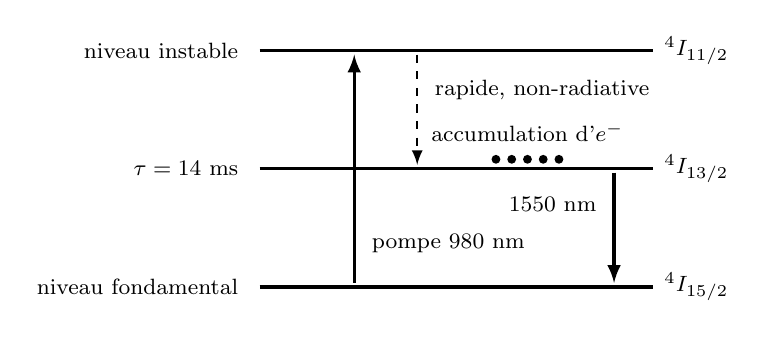
\begin{tikzpicture}[>=latex, every node/.style={font=\footnotesize}]
    % levels
    \draw[very thick] (0,0) -- (5,0) node[right] {$^4I_{15/2}$};
    \draw[very thick] (0,1.5) -- (5,1.5) node[right] {$^4I_{13/2}$};
    \draw[very thick] (0,3.0) -- (5,3.0) node[right] {$^4I_{11/2}$};
    \node[anchor=east, align=right] at (-0.15,3.0) {niveau instable};
    \node[anchor=east, align=right] at (-0.15,1.5) {$\tau=14$ ms};
    \node[anchor=east, align=right] at (-0.15,0) {niveau fondamental};
    % pump
    \draw[->, very thick] (1.2,0.05) -- (1.2,2.95);
    \node[anchor=west] at (1.3,0.55) {pompe 980 nm};
    % non-radiative
    \draw[->, thick, dashed] (2.0,2.95) -- (2.0,1.55);
    \node[anchor=west] at (2.1,2.5) {rapide, non-radiative};
    % lasing
    \draw[->, very thick] (4.5,1.45) -- (4.5,0.05);
    \node[anchor=east] at (4.4,1.05) {1550 nm};
    % accumulation dots
    \foreach \x in {3.0,3.2,...,3.8}{\fill (\x,1.62) circle (1.6pt);}
    \node[anchor=south] at (3.4,1.72) {accumulation d'$e^-$};
  \end{tikzpicture}
  \caption*{\footnotesize Système à 3 niveaux d'un amplificateur à fibre dopée
  erbium. The long durée de vie of $^4I_{13/2}$ is what gives the EDFA its
  transparence au débit.}
\end{figure}

\noindent On peut effectuer du pompage dans les différentes bandes
d'absorption de l'Erbium --- autour de 800 nm, autour de 980 nm et autour de
1480 nm. En pratique, on utilise l'absorption d'une onde à 980 nm fournie par
une diode laser puissante pour réaliser le pompage et l'émission radiative
s'effectue entre 1525 nm et 1565 nm. Une fibre dopée Erbium peut être
approximée par un système à trois niveaux. La transition
$^4I_{15/2}\to{}^4I_{11/2}$ permet d'absorber l'énergie d'une onde pompe à
980 nm. Les atomes sont donc transférés du niveau fondamental vers le niveau
excité. La transition $^4I_{11/2}\to{}^4I_{13/2}$ est très rapide et
non-radiative. Les atomes sont donc quasi-instantanément transférés vers le
niveau $^4I_{13/2}$ qui a une durée de vie très longue de 14 ms. Toutes les
conditions sont ainsi remplies pour obtenir une inversion de population entre
les niveaux $^4I_{13/2}$ et $^4I_{15/2}$ et donc une transition laser radiative
autour de 1550 nm permettant l'amplification à ces longueurs d'onde par
émission stimulée. Pour un gain suffisant, la fibre mesure une dizaine de
mètres et est lovée sur une bobine de 5 à 10 cm de diamètre.

\begin{conclusion}[Why the EDFA revolutionised optical telecommunications]
  Ce qui est intéressant pour les communications haut débit est la durée de vie
  de l'état $^4I_{13/2}$, très longue ($\tau=14$ ms), which corresponds to a
  bande passante $1/\tau\approx 70$ Hz. Cela rend cet amplificateur très peu
  réactif aux variations très rapides de la puissance d'entrée à amplifier,
  puisque cette constante de temps est directement reliée à la vitesse à
  laquelle est capable de varier la population de cet état --- and hence the
  gain. Ainsi, par exemple à 10 Gb/s, le gain de l'amplification est le même
  quelle que soit la valeur du bit d'entrée (0 ou 1). Le taux d'extinction
  $I_1/I_0$ n'est donc pas modifié aux hautes fréquences avec ce type
  d'amplificateur (hormis l'ajout d'un bruit) : on parle de
  \textbf{transparence au débit} (\textit{transparency to the bit rate}).
  L'EDFA est donc utilisé sur des transmissions haut débit, directement soudé à
  la fibre de transmission, tous les 100 km pour une liaison terrestre et tous
  les 50 à 70 km pour les transmissions sous-marines.
\end{conclusion}

\paragraph{L'amplificateur à semiconducteur}
Le fonctionnement de ce type d'amplificateur se modélise par un système à deux
niveaux associé à un pompage électronique. D'une manière générale, ce qu'il
faut retenir est que la durée de vie des porteurs dans la bande de conduction
est \emph{beaucoup plus rapide} que pour l'Erbium. Elle est de l'ordre de la
nanoseconde ou du dixième de nanoseconde, so a bande passante of a few GHz. Les
populations peuvent donc varier entre les 1 et les 0 d'un signal à 10 Gb/s
entrainant une modification du gain rapide et donc des distorsions du signal
entrant. On dit que son fonctionnement est \emph{non-linéaire}. Ce type
d'amplificateur n'est donc pas (ou peu) utilisé pour les amplificateurs optiques
en ligne sur de longues distances. Par contre, il est utilisé pour réaliser des
fonctions optiques : commutation, traitement du signal, etc. et depuis peu pour
le réseau d'accès.

On the other hand its gain per unit length is several orders of magnitude above
erbium's, so un amplificateur à semiconducteur d'une longueur de quelques
millimètres permet d'avoir le même gain qu'un EDFA pour lequel la fibre doit
avoir une longueur d'une dizaine de mètres. L'amplificateur à semiconducteur est
donc bien plus intégrable qu'un EDFA; a packaged device is about 2 cm.

\subsection{Le laser : le milieu amplificateur plongé dans une cavité résonante}
Nous avons vu comment on pouvait obtenir un milieu amplificateur. Pour obtenir
un laser, il suffit de placer ce milieu amplificateur dans une cavité résonante
et de respecter certaines conditions. Le fait de faire aller et venir la lumière
dans le milieu amplificateur à l'aide d'une cavité optique permet d'augmenter
considérablement la capacité d'amplification d'une onde puisque celle-ci va
transiter plusieurs fois dans le milieu. Ce facteur d'amplification élevé peut
compenser la perte d'énergie due à l'émission d'énergie vers l'extérieur,
indispensable si l'on veut que de la lumière sorte du laser. Toutes sortes de
cavités : miroirs plan / plan (cavité Fabry--Perot), miroirs plan / concave, en
anneau, à fibre.

\subsubsection{La cavité résonante}
La façon la plus simple pour expliquer le principe de fonctionnement d'une
cavité résonante est de considérer la cavité Fabry--Perot constituée de deux
miroirs plans, face à face, avec $r_1,r_2$ les facteurs de réflexion en
amplitude de chaque miroir et $t_1,t_2$ les facteurs de transmission
correspondants. Dans ce type de cavité, les réflexions successives sur chaque
miroir vont engendrer des interférences entre un grand nombre d'ondes
cohérentes --- un problème d'interférences à ondes multiples.

\begin{prop}[Sélectivité spectrale (\textit{wavelength selectivity})]
  Si le déphasage accumulé sur un aller-retour est un multiple de $2\pi$, les
  ondes s'ajoutent en phase, le champ est alors transmis par la cavité. If the
  phase is offset by $\pi$, the ondes superpose in phase opposition, the field
  cancels and is no longer transmitted. Une telle cavité résonante est donc
  \emph{sélective en longueur d'onde} comme une corde de guitare.
\end{prop}

\noindent Si on note $\psi_0$ l'amplitude complexe d'une onde plane incidente
(with $e$ the cavity length, filled with index $n$), les amplitudes complexes
des ondes transmises après un nombre d'allers-retours successifs s'écrivent :
\[\psi_1=t_1t_2\psi_0e^{i\varphi/2},\quad
  \psi_2=r_1r_2t_1t_2\psi_0e^{i\varphi}e^{i\varphi/2},\quad
  \psi_3=r_1^2r_2^2t_1t_2\psi_0e^{i2\varphi}e^{i\varphi/2},\quad\ldots\]
où
\[\varphi=\frac{2\pi}{\lambda_0}\,2ne\]
désigne la différence de phase accumulée par une onde sur un aller-retour. Si on
introduit les facteurs de réflexion et de transmission en intensité de chacun
des miroirs, en prenant pour simplifier les calculs $r=r_1=r_2$ et $t=t_1=t_2$ :
$R=r^2$ et $T=t^2$. L'amplitude complexe de l'onde transmise au point $P$ du
plan focal de la lentille de collection est la somme des amplitudes complexes des ondes
transmises :
\[\psi_t(P)=\sum_i\psi_i
  =T\psi_0\left[1+Re^{i\varphi}+R^2e^{i2\varphi}+\cdots+R^me^{im\varphi}
  +\cdots\right]e^{i\varphi/2}.\]
C'est une suite géométrique de raison $Re^{i\varphi}$. Puisque $R<1$, on trouve
après sommation :
\[\psi_t(P)=T\psi_0\,\frac{1}{1-Re^{i\varphi}}\,e^{i\varphi/2},\]
et l'intensité de l'onde transmise résulte immédiatement de l'équation
précédente :
\[I_t(P)\propto\left|\psi_t(P)\right|^2
  =\frac{I_{max}}{1+M\sin^2\dfrac{\varphi}{2}},\qquad
  M=\frac{4R}{(1-R)^2},\qquad
  I_{max}=I_0\left(\frac{T}{1-R}\right)^2.\]

\begin{definition}[Fonction d'Airy]
  La fonction
  \[A(\varphi)=\frac{1}{1+M\sin^2\dfrac{\varphi}{2}}\]
  est appelée \textbf{fonction d'Airy} (\textit{Airy function}). C'est une
  fonction paire, symétrique. Chaque pic est appelé \textbf{mode longitudinal}
  (\textit{longitudinal mode}) de la cavité.
\end{definition}

Pour $\varphi$ petit devant $\pi$ (autour du pic centré autour de
$\varphi=0\ [2\pi]$), on peut écrire que :
\[A(\varphi)=\frac{1}{1+M\sin^2\left(\varphi/2\right)}
  \approx\frac{1}{1+M\left(\varphi/2\right)^2},\]
on reconnaît l'expression d'une lorentzienne : la fonction d'Airy est donc
constituée d'une succession de pics dont le profil est lorentzien.
L'interférence de ces ondes sera constructive et maximale si et seulement si $R$
est voisin de 1. Les très bons lasers possèdent des facteurs de réflexion en
amplitude des deux miroirs en valeur absolue proches de 1, les ondes véhiculées
par les différents rayons transmis ont alors pratiquement la même amplitude. Par
contre, les lasers à semiconducteur peuvent se permettre d'avoir des facteurs de
réflexion de l'ordre de 30\% seulement car le gain est très fort.

\begin{figure}[h!]
  \centering
  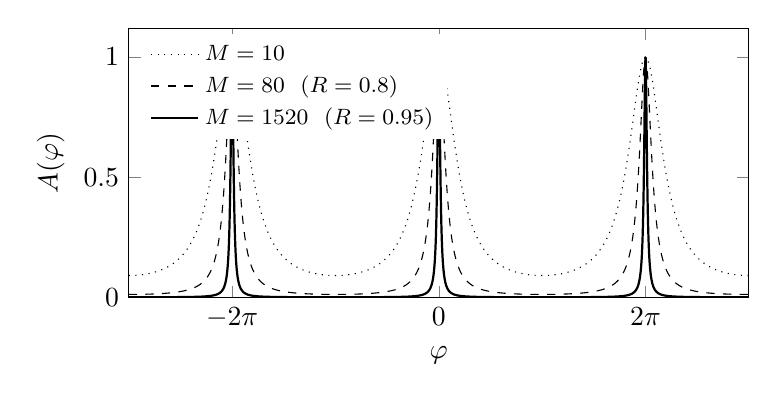
\begin{tikzpicture}
    \begin{axis}[width=0.78\textwidth, height=5cm,
      xlabel={$\varphi$}, ylabel={$A(\varphi)$},
      xmin=-1.5, xmax=1.5, ymin=0, ymax=1.12,
      xtick={-1,0,1}, xticklabels={$-2\pi$,$0$,$2\pi$},
      ytick={0,0.5,1},
      legend style={draw=none, font=\footnotesize, at={(0.02,0.98)},
        anchor=north west},
      legend cell align=left, samples=2400]
      \addplot[black, dotted, domain=-1.5:1.5] {1/(1+10*(sin(180*x))^2)};
      \addlegendentry{$M=10$}
      \addplot[black, dashed, domain=-1.5:1.5] {1/(1+80*(sin(180*x))^2)};
      \addlegendentry{$M=80$ \ ($R=0.8$)}
      \addplot[black, thick, domain=-1.5:1.5] {1/(1+1520*(sin(180*x))^2)};
      \addlegendentry{$M=1520$ \ ($R=0.95$)}
    \end{axis}
  \end{tikzpicture}
  \caption*{\footnotesize La fonction d'Airy est représentée pour trois valeurs
  de $M$. Plus $R$ augmente, plus les pics sont fins. Successive peaks are
  separated by the intervalle spectral libre $c/2ne$.}
\end{figure}

\paragraph{Largeur d'un mode}
On détermine la largeur totale à mi-hauteur en résolvant $A(\varphi)=0.5$ :
\[\Delta\varphi_{1/2}=\frac{4}{\sqrt{M}}=\frac{2(1-R)}{\sqrt{R}}.\]
Ainsi, plus $R$ augmente, plus la largeur des pics diminue. Application
numérique : pour $R=0.8$, $M=80$ et $\Delta\varphi_{1/2}\approx 0.45$ ; pour
$R=0.95$, $M=1520$ et $\Delta\varphi_{1/2}\approx 0.1$.

Rather than in phase, on peut convertir l'axe en longueur d'onde. Puisque
$\varphi_{AR}=2\pi\,2ne/\lambda_0$, alors
$\Delta\varphi=2\pi\,2ne\,\Delta\lambda/\lambda_0^2$, soit la largeur à
mi-hauteur exprimée en mètres :
\[\Delta\lambda_{1/2}=\frac{\lambda_0^2}{2\pi\,2ne}\,\Delta\varphi_{1/2}
  =\frac{\lambda_0^2}{2\pi\,2ne}\,\frac{2(1-R)}{\sqrt{R}}.\]

\begin{example}[Orders of magnitude]
  Si $\lambda_0=0.5\ \mu$m, $e=1$ cm et $n=1$ : pour $R=0.8$,
  $\Delta\lambda_{1/2}=0.89$ pm ; pour $R=0.95$, $0.2$ pm ; et pour $R=0.99$,
  $0.04$ pm. A Fabry--Perot cavity is an extraordinarily fine filter.
\end{example}

\begin{definition}[Intervalle spectral libre]
  L'espacement entre les pics de la fonction d'Airy, appelé
  \textbf{intervalle spectral libre} (\textit{free spectral range}), vaut
  \[\mathrm{ISL}=\frac{c}{2ne}.\]
\end{definition}

\begin{remark}[Confinement means quantisation]
  The mechanism is general: confining an onde quantises something. Corde
  vibrante : confinement longitudinal, quantification des fréquences (comme la
  cavité résonante optique). Fibre optique : confinement transverse,
  quantification de $k_x$ dans la direction de confinement (angles permis) ;
  il existe également un confinement angulaire. Électron dans un puits de
  potentiel : confinement autour de l'atome, quantification des énergies.
\end{remark}

\subsubsection{Le laser}
Le laser est constitué d'un milieu amplificateur inséré dans une cavité
résonante. Plaçons-nous dans le cas d'une cavité à miroirs plans parallèles
appelée cavité Fabry--Perot. Considérons une onde (provenant de l'émission
spontanée) qui prend naissance dans le milieu amplificateur. Au fur et à mesure
de sa propagation, elle va stimuler un certain nombre de transitions et s'en
trouver amplifiée. Si la direction est normale aux miroirs, l'onde émise est
renvoyée dans le milieu amplificateur où elle effectue un certain nombre
d'allers-retours entrecoupés de réflexions.

\begin{figure}[h!]
  \centering
  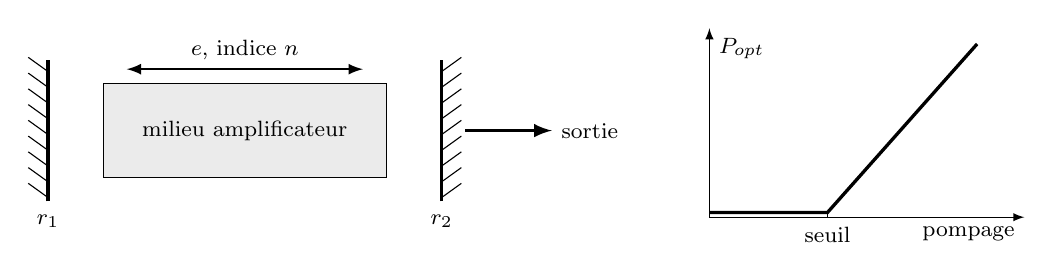
\begin{tikzpicture}[>=latex, every node/.style={font=\footnotesize}]
    % mirrors
    \draw[very thick] (0,-0.9) -- (0,0.9);
    \draw[very thick] (5,-0.9) -- (5,0.9);
    \foreach \y in {-0.85,-0.65,...,0.85}{
      \draw (0,\y) -- (-0.25,\y+0.18);
      \draw (5,\y) -- (5.25,\y+0.18);}
    \draw[fill=black!8] (0.7,-0.6) rectangle (4.3,0.6);
    \node at (2.5,0) {milieu amplificateur};
    \draw[<->, thick] (1.0,0.78) -- (4.0,0.78);
    \node[anchor=south] at (2.5,0.78) {$e$, indice $n$};
    \node[anchor=north] at (0,-0.95) {$r_1$};
    \node[anchor=north] at (5,-0.95) {$r_2$};
    \draw[->, very thick] (5.3,0) -- (6.4,0);
    \node[anchor=west] at (6.4,0) {sortie};
    % threshold curve
    \begin{scope}[xshift=8.4cm, yshift=-1.1cm]
      \draw[->] (0,0) -- (4.0,0) node[anchor=north east] {pompage};
      \draw[->] (0,0) -- (0,2.4) node[anchor=north west] {$P_{opt}$};
      \draw[very thick] (0,0.06) -- (1.5,0.06) -- (3.4,2.2);
      \draw[dashed] (1.5,0) -- (1.5,0.06);
      \node[anchor=north] at (1.5,0) {seuil};
    \end{scope}
  \end{tikzpicture}
  \caption*{\footnotesize Left: le milieu amplificateur plongé dans une cavité
  résonante. Right: existence d'un seuil --- below it the laser emits only
  émission spontanée amplifiée filtrée.}
\end{figure}

\begin{prop}[Les deux conditions d'oscillation]
  Pour que l'onde continue à croître, il faut que le gain compense les pertes
  dues aux réflexions et à l'absorption du milieu et des miroirs. Il faut
  également qu'après un aller-retour, l'onde revienne en phase avec elle-même :
  si elle est en phase, il va y avoir des interférences constructives et
  l'oscillation ainsi que l'amplification vont se poursuivre ; si elle n'est pas
  en phase, les interférences destructives vont rajouter des pertes qui feront
  que la condition de gain ne sera plus respectée. Hence the two
  \textbf{conditions de seuil d'oscillation} (\textit{oscillation threshold
  conditions}):
  \[\text{gain condition:}\quad
    \text{Gain}_{\text{round trip}}=\text{Losses}_{\text{round trip}},\qquad
    \text{phase condition:}\quad
    \varphi_{\text{round trip}}=2k\pi,\ k\in\zee.\]
\end{prop}

\begin{conclusion}
  La première, imposant un gain minimum, détermine l'\emph{inversion de
  population} nécessaire. La seconde, fixant la rotation de phase de l'onde
  oscillante lors d'un aller et retour, justifie l'introduction des \emph{modes}
  de la cavité, et impose la fréquence exacte d'oscillation.
\end{conclusion}

Lorsque la condition de gain est respectée, toute onde de fréquence proche de
celle du centre de la raie et cheminant parallèlement à l'axe de la cavité, voit
son amplitude accrue après une traversée et une réflexion et peut
potentiellement « laser ». Cependant, as the fonction d'Airy shows, toutes les
fréquences optiques ne peuvent pas osciller dans la cavité.

\begin{figure}[h!]
  \centering
  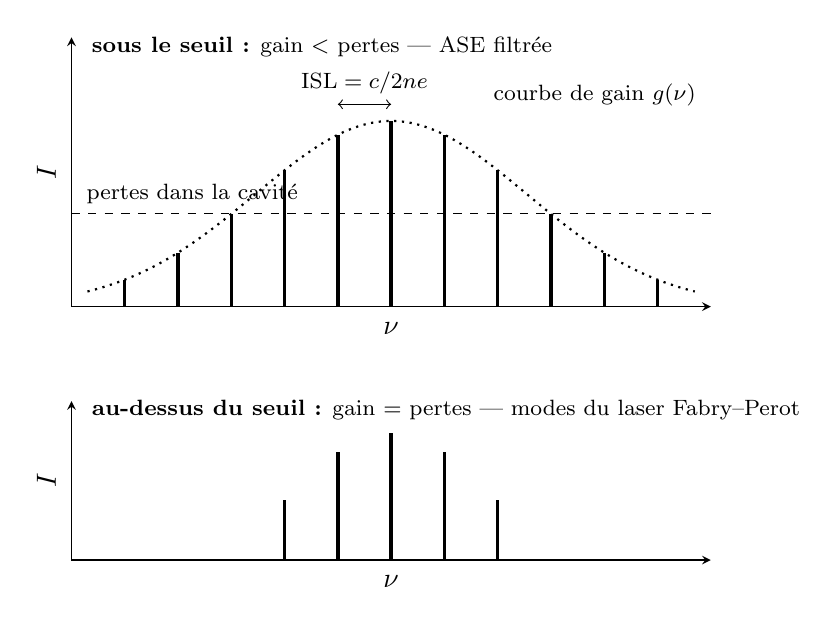
\begin{tikzpicture}
    \begin{axis}[name=top, width=0.8\textwidth, height=5cm,
      xmin=0, xmax=12, ymin=0, ymax=1.45,
      xlabel={$\nu$}, ylabel={$I$}, xtick=\empty, ytick=\empty,
      axis lines=left, clip=false]
      \addplot[black, dotted, thick, domain=0.3:11.7, samples=120]
        {exp(-((x-6)/3.6)^2)};
      \node[font=\footnotesize, anchor=east] at (axis cs:11.9,1.14)
        {courbe de gain $g(\nu)$};
      \addplot[black, dashed, domain=0:12, samples=2] {0.5};
      \node[font=\footnotesize, anchor=south west] at (axis cs:0.1,0.5)
        {pertes dans la cavité};
      \addplot[black, ycomb, very thick] coordinates
        {(1,0.145) (2,0.291) (3,0.499) (4,0.734) (5,0.926) (6,1.0)
         (7,0.926) (8,0.734) (9,0.499) (10,0.291) (11,0.145)};
      \draw[<->] (axis cs:5,1.09) -- (axis cs:6,1.09);
      \node[font=\footnotesize, anchor=south] at (axis cs:5.5,1.09)
        {$\mathrm{ISL}=c/2ne$};
      \node[font=\footnotesize, anchor=west] at (axis cs:0.2,1.40)
        {\textbf{sous le seuil :} gain $<$ pertes --- ASE filtrée};
    \end{axis}
    \begin{axis}[at={(0cm,-1.2cm)}, anchor=north west,
      width=0.8\textwidth, height=3.6cm,
      xmin=0, xmax=12, ymin=0, ymax=1.25,
      xlabel={$\nu$}, ylabel={$I$}, xtick=\empty, ytick=\empty,
      axis lines=left, clip=false]
      \addplot[black, ycomb, very thick] coordinates
        {(4,0.47) (5,0.85) (6,1.0) (7,0.85) (8,0.47)};
      \node[font=\footnotesize, anchor=west] at (axis cs:0.2,1.18)
        {\textbf{au-dessus du seuil :} gain $=$ pertes --- modes du laser Fabry--Perot};
    \end{axis}
  \end{tikzpicture}
  \caption*{\footnotesize Construction of the spectrum of a Fabry--Perot laser.
  Only the modes whose gain compensates the losses survive.}
\end{figure}

Sur la courbe du haut, on peut observer la courbe d'émission spontanée filtrée
par la fonction de transmission de la cavité Fabry--Perot --- la fonction
d'Airy --- dont l'espacement entre les pics est l'intervalle spectral libre
$\mathrm{ISL}=c/2ne$. On peut également observer la valeur des pertes par
aller-retour. La courbe du bas montre le spectre d'émission d'un laser
Fabry--Perot quand le pompage augmente : les pics laser ne sont émis qu'aux
fréquences pour lesquelles le gain est compensé par les pertes : ces pics sont
appelés \textbf{modes longitudinaux du laser}.

\begin{remark}
  Le spectre d'émission d'un laser Fabry--Perot est \emph{a priori multimode}.
  Pour qu'il devienne monomode, il faudrait augmenter les pertes pour les modes
  que l'on souhaite supprimer. Ceci peut être réalisé par exemple à l'aide de
  miroirs sélectifs en longueur d'onde.
\end{remark}

\begin{example}[Switching a laser on]
  The sequence is: allumage du laser, génération de photons spontanés ; si
  photon spontané dans la direction perpendiculaire aux miroirs, amplification
  du photon spontané ; réflexion sur les miroirs ; si longueur d'onde du photon
  spontané pas adaptée à la cavité, interférences destructives, extinction de
  l'onde ; si longueur d'onde du photon spontané adaptée à la cavité,
  l'amplification continue : oscillations.
\end{example}

\subsubsection{Caractéristiques principales d'un faisceau laser}
Les propriétés d'un laser sont très différentes de la lumière « naturelle »
produite par exemple par le soleil ou les lampes à incandescence. Une lampe à
incandescence peut fournir de manière continue une puissance de l'ordre du kW,
dont le spectre en longueur d'onde s'étale sur plusieurs centaines de
nanomètres. Ses longueurs de cohérence spatiale et temporelle sont très
faibles : la longueur de cohérence d'une lumière blanche s'étalant de 0.4 à
0.8 $\mu$m est de l'ordre de 0.8 $\mu$m. De plus, cette lumière n'est pas
polarisée.

\begin{remark}
  On considérera en première approximation que la longueur de cohérence
  correspond à la longueur du train d'onde.
\end{remark}

\paragraph{La monochromaticité de son rayonnement}
La « couleur » de la lumière émise est extrêmement pure, elle correspond à une
onde quasi-sinusoïdale de fréquence située dans le domaine optique
($10^{14}$ Hz). La lumière laser est une association de photons aux propriétés
très voisines --- dans le même état quantique : les photons ne respectent pas le
principe d'exclusion de Pauli --- conséquence intrinsèque de l'émission
stimulée et du filtrage opéré par la cavité. Cette uniformité des photons est
traduite par la notion de \textbf{cohérence temporelle} (\textit{temporal
coherence}) du faisceau, dans laquelle résident toutes les propriétés
remarquables d'une telle source. The longueur de cohérence follows the
linewidth as $L_c=c/\Delta\nu$:

\begin{center}
  \begin{tabular}{lccc}
    \toprule
    $\Delta\nu$ & 1 MHz & 1 kHz & 1 Hz \\
    \midrule
    $L_{\text{coherence}}$ & 300 m & 300 km & 300\,000 km \\
    \bottomrule
  \end{tabular}
\end{center}

\begin{example}
  La longueur de cohérence d'un laser He--Ne de largeur de raie 1.5 GHz est de
  0.2 m et peut atteindre 30 km pour un laser CO$_2$ d'une largeur de raie égale
  à 10 kHz. Notons également plus récemment la réalisation de lasers
  fonctionnant dans le visible (563 nm) et dont la largeur de raie est
  \emph{sub-hertzienne}. Where natural light has a train d'onde a few
  micrometres long, a laser's runs from a few centimetres to a kilometre.
\end{example}

\begin{example}[VIRGO]
  Projet VIRGO : interféromètres pour mesure d'ondes gravitationnelles. Passage
  d'une onde gravitationnelle : déformation d'un milliardième de milliardième de
  mètre dans les bras de 3 km de Virgo --- moins d'un millième de la taille d'un
  proton --- for a source emitting some $3.6\cdot10^{49}$ W. Noise is the whole
  problem, and the measurement is only conceivable with a source of that
  monochromaticity.
\end{example}

\paragraph{La cohérence spatiale de son rayonnement}
Toute la puissance lumineuse peut être concentrée dans un mode de propagation.
C'est ce que l'on appelle la \textbf{cohérence spatiale} (\textit{spatial
coherence}). Le rayonnement laser est focalisable sur de très petites surfaces,
down to the order of $\lambda$. Des densités exceptionnelles de puissance allant
jusqu'à plusieurs mégawatts par mm$^2$ sont possibles.

\begin{remark}
  Being focusable is not the same as being directive. Un faisceau laser n'est
  pas très directif, because of diffraction: a semiconductor laser with an
  emitting zone a few micrometres across diverges by 30 to 60 degrees.
  L'amplification \emph{interne} est très directive, along the cavity axis,
  which is why the amplification is so efficient.
\end{remark}

\paragraph{Des impulsions ultra-courtes}
Localisation temporelle de l'énergie lumineuse : la durée des impulsions de
lumière produites peut être réduite à quelques $10^{-17}$ s (10 attosecondes,
record). Dans ce cas, la source est alors très large spectralement à cause du
principe de Heisenberg. Seuls les lasers continus ont des spectres ultrafins.

\begin{example}
  Laser Mégajoule : durée 20 ns, énergie mégajoule, combinaison de 240
  faisceaux laser fournissant 7.5 kJ chacun --- fusion thermonucléaire. In
  machining, drilling with a femtosecond laser gives a far cleaner hole than a
  nanosecond laser --- la découpe au laser femtoseconde est plus « propre » ---
  which matters for cutting and for surgery of the eye and the brain. Grâce au
  large spectre du continuum d'une source impulsionnelle, on peut même détecter
  plusieurs espèces à la fois (LIDAR), and a Doppler frequency shift gives the
  wind.
\end{example}

\paragraph{Des émissions chaotiques}
A laser can also be driven into a chaotic regime, which is used for private
communications in the mid-infrared, built on photonic chaos with lasers à
cascade quantique in the fenêtre atmosphérique moyen IR, 9--11 $\mu$m.
Pourquoi : rayonnement infrarouge moyen furtif, imprévisibilité du chaos, mise
en œuvre simple. La génération du chaos $C$ est basée sur le signal d'entrée,
donc seul le récepteur qui connaît la façon dont le chaos est généré peut
reproduire le chaos et l'annuler pour récupérer le signal $M$: with a slave
laser regenerating $C'$,
\[M+C-C'=M'\approx M,\qquad C-C'\ll 1,\]
which assumes matched parameters --- or a very small mismatch --- between the two
physical systems, for the chaos to synchronise. Records : 120 km sur fibre
optique et 35 m en espace libre.

\paragraph{La polarisation de son rayonnement}
La nature même de l'émission laser n'oblige pas la lumière laser à être
polarisée. Par contre, il est difficile de supprimer tous les éléments
polarisants dans une cavité. Pour cela, la plupart des lasers sont polarisés
même si en prenant des précautions, on peut faire en sorte qu'ils ne le soient
pas.

\begin{conclusion}[What separates the three emission mechanisms]
  Rayonnement thermique is incoherent, emitted in all directions, over a
  spectre continu several hundred THz wide. Émission spontanée ---
  luminescence --- is also incoherent and emitted in all directions, but it is
  quantised and its spectrum is only a few nanometres wide. Émission stimulée
  clones the incident photon in phase, frequency, direction and polarisation;
  placed in a resonant cavity that filters it and fed by a pompage strong enough
  to invert the populations, it gives a source that is coherent in time and in
  space, monochromatique down to the sub-hertz, and focusable to the longueur
  d'onde.
\end{conclusion}
